\documentclass[aspectratio=169,10pt,t]{beamer}
\usepackage[utf8]{inputenc}
\usepackage[T1]{fontenc}
\usepackage[spanish,es-tabla,es-nodecimaldot]{babel}
\usepackage{lmodern}
\usepackage{amsmath,amssymb,booktabs,array}
\usepackage{graphicx}
\usepackage[table]{xcolor}
\usepackage{tikz}
\usetikzlibrary{positioning,arrows.meta,calc,shapes.geometric,fit}
\usepackage[most]{tcolorbox}
\usepackage{hyperref}
\usepackage{microtype}
\usepackage{ragged2e}
\hyphenpenalty=10000 \exhyphenpenalty=10000 \emergencystretch=2em
\definecolor{Ink}{HTML}{17263D}
\definecolor{Blue}{HTML}{006B91}
\definecolor{Sky}{HTML}{DDF0F6}
\definecolor{Turq}{HTML}{11A6B4}
\definecolor{Gold}{HTML}{E5A43B}
\definecolor{Warn}{HTML}{A85A24}
\definecolor{Muted}{HTML}{66778C}
\definecolor{Paper}{HTML}{FAFCFE}
\definecolor{Pale}{HTML}{EFF5F8}
\definecolor{Green}{HTML}{2D8066}
\setbeamercolor{normal text}{fg=Ink,bg=Paper}
\setbeamercolor{frametitle}{fg=Ink,bg=Paper}
\setbeamercolor{structure}{fg=Blue}
\setbeamercolor{alerted text}{fg=Warn}
\setbeamertemplate{navigation symbols}{}
\setbeamertemplate{itemize item}{\raisebox{.12ex}{\scriptsize\textcolor{Turq}{$\blacktriangleright$}}}
\setbeamertemplate{itemize subitem}{\raisebox{.12ex}{\scriptsize\textcolor{Blue}{$\bullet$}}}
\setbeamertemplate{frametitle}{\vspace{0.19cm}\hspace{0.32cm}\parbox{0.85\paperwidth}{\Large\bfseries\insertframetitle\par\vspace{0.05cm}{\color{Turq}\rule{1.45cm}{1.7pt}}}\vspace{-0.28cm}}
\setbeamertemplate{footline}{%
\begin{tikzpicture}[remember picture,overlay]
  \fill[Blue] (current page.south west) rectangle ([yshift=0.16cm]current page.south east);
  \node[anchor=south west,text=Muted,font=\tiny] at ([xshift=0.4cm,yshift=0.22cm]current page.south west) {RL BENCHMARK LAB \quad | \quad PROYECTO 01 · AGENTES INTELIGENTES};
  \node[anchor=south east,text=Muted,font=\tiny] at ([xshift=-0.38cm,yshift=0.22cm]current page.south east) {\insertframenumber\,/\,\inserttotalframenumber};
\end{tikzpicture}\vspace{0.34cm}}
\setbeamertemplate{blocks}[rounded][shadow=false]
\setbeamercolor{block title}{bg=Sky,fg=Blue}
\setbeamercolor{block body}{bg=Pale,fg=Ink}
\newtcolorbox{info}[1][]{enhanced,before upper={\RaggedRight},colback=Pale,colframe=Sky,arc=2mm,boxrule=.65pt,left=2.4mm,right=2.4mm,top=1.5mm,bottom=1.5mm,#1}
\newtcolorbox{takeaway}[1][]{enhanced,before upper={\RaggedRight},colback=white,colframe=Turq,boxrule=1pt,arc=2mm,left=2.5mm,right=2.5mm,top=1.8mm,bottom=1.8mm,#1}
\newcommand{\metric}[2]{\begin{minipage}[t]{.28\linewidth}\centering{\color{Blue}\LARGE\bfseries #1}\\[-.05cm]{\color{Muted}\scriptsize #2}\end{minipage}}
\hypersetup{colorlinks=true,urlcolor=Blue,linkcolor=Blue,pdftitle={Aprendizaje por refuerzo: Q-learning, DQN y Double DQN},pdfauthor={Kevin Erazo, Steven Rodríguez},pdflang={es}}
\title{Aprendizaje por refuerzo: Q-learning, DQN y Double DQN}
\subtitle{Evaluación reproducible en CartPole-v1 y Acrobot-v1}
\author{Kevin Erazo \and Steven Rodríguez}
\institute{Agentes Inteligentes · Proyecto 01}
\date{Noviembre de 2026}
\begin{document}
% PRESENTACIÓN RESUMIDA: 10 diapositivas / 10 minutos
% Compilar con: pdflatex (2 veces). Requiere la carpeta figs/ junto a este archivo.
% 1 — 0:35
\begin{frame}[plain]
\begin{tikzpicture}[remember picture,overlay]
  \fill[Paper] (current page.south west) rectangle (current page.north east);
  \fill[Blue] (current page.north west) rectangle ([xshift=.17cm]current page.south west);
  \fill[Sky] ([xshift=11.25cm,yshift=-.85cm]current page.north west) circle (2.6cm);
  \fill[Turq,opacity=.17] ([xshift=12.45cm,yshift=-1.4cm]current page.north west) circle (1.7cm);
  \draw[Turq,line width=2.4pt] ([xshift=10.4cm,yshift=-7.9cm]current page.north west)
   -- ([xshift=11.5cm,yshift=-7.0cm]current page.north west)
   -- ([xshift=12.8cm,yshift=-7.5cm]current page.north west)
   -- ([xshift=14.9cm,yshift=-5.7cm]current page.north west);
  \foreach \x/\y in {10.4/-7.9,11.5/-7.0,12.8/-7.5,14.9/-5.7}
    \fill[Blue] ([xshift=\x cm,yshift=\y cm]current page.north west) circle (.09cm);
\end{tikzpicture}
\vspace{.55cm}
{\color{Turq}\large PROYECTO 01 · AGENTES INTELIGENTES}\par\vspace{.34cm}
{\color{Ink}\fontsize{26}{31}\selectfont\bfseries Aprendizaje por refuerzo\\[.07cm] Q-learning, DQN y Double DQN}\par\vspace{.24cm}
{\color{Muted}\large Comparación experimental en CartPole y Acrobot}\par\vspace{.65cm}
{\large\bfseries Kevin Erazo \qquad Steven Rodríguez}\par\vspace{.16cm}
{\small\color{Muted}33 entrenamientos reales · 4,5 millones de interacciones}\par\vspace{.31cm}
{\footnotesize\color{Blue}\url{https://github.com/Steven735-star/rl-benchmark-lab}}
\end{frame}

% 2 — 0:55
\begin{frame}{Problema y preguntas de investigación}
\begin{columns}[T,onlytextwidth]
\column{.54\textwidth}
\begin{info}
\textbf{¿Mayor complejidad implica mejor aprendizaje?}\par\vspace{.09cm}
\small Comparamos métodos tabulares y redes profundas, observando desempeño final y estabilidad entre ejecuciones independientes.
\end{info}
\vspace{.16cm}
\begin{itemize}\RaggedRight\setlength{\itemsep}{.10cm}
\item \textbf{RQ1:} ¿Cómo influye discretizar el estado con 6, 10 o 20 intervalos frente a DQN?
\item \textbf{RQ2:} ¿Cómo afectan learning rate, exploración y red objetivo a DQN?
\item \textbf{RQ3:} ¿Double DQN mejora el resultado y su consistencia?
\end{itemize}
\column{.44\textwidth}
\begin{info}
{\large\bfseries CartPole-v1}\par\vspace{.08cm}
\small 4 observaciones continuas · 2 acciones\par
\small Equilibrar una barra · retorno objetivo \textbf{\textcolor{Blue}{$\geq475$}}.
\end{info}
\vspace{.15cm}
\begin{info}
{\large\bfseries Acrobot-v1}\par\vspace{.08cm}
\small 6 observaciones continuas · 3 acciones\par
\small Impulsar el sistema hasta la altura meta · objetivo \textbf{\textcolor{Blue}{$\geq-100$}}.
\end{info}
\end{columns}

\end{frame}

% 3 — 1:10
\begin{frame}{Algoritmos: de la tabla a Double DQN}
\begin{columns}[T,onlytextwidth]
\column{.48\textwidth}
\begin{info}
\textbf{Q-learning tabular}\par\vspace{.08cm}
\small Discretiza las 4 observaciones de CartPole y actualiza una tabla de valores de acciones.\par\vspace{.12cm}
\small $\delta=r+\gamma(1-d)\max_{a'}Q(s',a')-Q(s,a)$\par\vspace{.04cm}\small $Q(s,a)\leftarrow Q(s,a)+\alpha\,\delta$\par\vspace{.12cm}
\small $6^4=1.296$; $10^4=10.000$; $20^4=160.000$ estados. 
\end{info}
\vspace{.15cm}
\begin{info}
\textbf{DQN}\par\vspace{.07cm}
\small Reemplaza la tabla por una red MLP \textbf{128–128 ReLU}, entrenada con \emph{experience replay} y una \emph{target network}. 
\end{info}
\column{.49\textwidth}
\begin{info}
\textbf{Double DQN}\par\vspace{.07cm}
\small Separa \emph{selección} y \emph{evaluación} de la próxima acción para reducir el sesgo de maximización:\par\vspace{.12cm}
\small $a^*=\arg\max_{a'}Q_{\theta}(s',a')$\par\vspace{.05cm}
\small $y=r+\gamma(1-d)Q_{\theta^-}(s',a^*)$.
\end{info}
\vspace{.15cm}
\begin{takeaway}
\small \textbf{Parámetros principales:} $\gamma=0{,}99$; DQN con Adam LR $5\cdot10^{-4}$, \emph{replay} de 50.000 transiciones, batch 64 y copia de la red objetivo cada 1.000 pasos.
\end{takeaway}
\end{columns}
\end{frame}

% 4 — 0:55
\begin{frame}{Diseño experimental y evaluación justa}
\centering\renewcommand{\arraystretch}{1.17}\small
\begin{tabular}{p{1.3cm}p{7.6cm}rr}
\toprule
\textbf{Bloque} & \textbf{Configuraciones} & \textbf{Corridas} & \textbf{Pasos/corrida} \\
\midrule
\textbf{Tier 1} & CartPole: Q-learning con 6, 10 y 20 bins; DQN & 12 & 200.000 \\
\textbf{Tier 2} & Acrobot: DQN base; LR baja/alta; $\epsilon$ corto/largo; sin target & 18 & 100.000 \\
\textbf{Tier 3} & Acrobot: Double DQN frente al DQN base & 3 & 100.000 \\
\bottomrule
\end{tabular}
\vspace{.24cm}
\begin{takeaway}\centering
\metric{11}{configuraciones}\hfill\metric{33}{ejecuciones}\hfill\metric{4,5 M}{pasos de entrenamiento}
\end{takeaway}
\vspace{.19cm}
\begin{info}
\small \textbf{Control experimental:} semillas 0, 1 y 2; presupuesto fijo por bloque. \textbf{Evaluación:} cada 10.000 pasos (10 episodios greedy) y al final (100 episodios greedy por semilla).
\end{info}
\end{frame}

% 5 — 1:20
\begin{frame}{Tier 1 · CartPole: Q-learning frente a DQN}
\begin{columns}[T,onlytextwidth]
\column{.60\textwidth}
\centering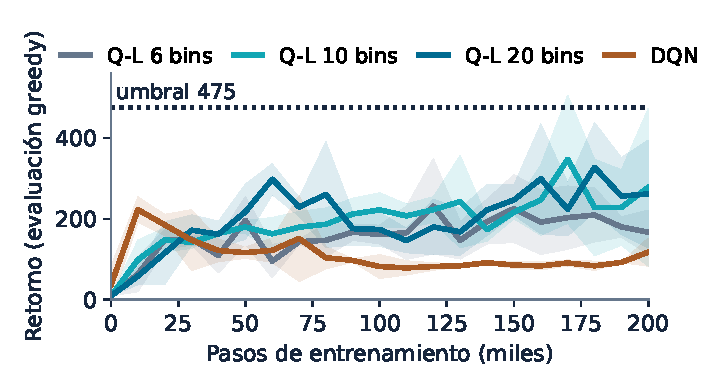
\includegraphics[width=\linewidth,height=.50\textheight,keepaspectratio]{figs/fig_cartpole.pdf}\par\vspace{.05cm}
{\color{Muted}\scriptsize Evaluaciones periódicas (10 episodios): media $\pm$ DE entre 3 semillas.}
\column{.38\textwidth}
\footnotesize
\renewcommand{\arraystretch}{1.19}
\begin{tabular}{@{}lrr@{}}\toprule
\textbf{Método} & \textbf{Media final} & \textbf{Éxitos} \\\midrule
Q-L, 6 bins & 161,80 & 0/3\\
Q-L, 10 bins & 275,68 & 1/3\\
\rowcolor{Sky!45}\textbf{Q-L, 20 bins} & \textbf{280,87} & 0/3\\
DQN & 117,46 & 0/3\\\bottomrule
\end{tabular}
\vspace{.15cm}
\begin{info}
\small DQN alcanzó \textbf{222,80} de media periódica a los 10.000 pasos, pero terminó con solo \textbf{117,46} en la evaluación final.
\end{info}
\end{columns}
\vspace{.18cm}
\begin{takeaway}\small\textbf{Hallazgo:} 20 bins produjo la mejor media; 10 bins obtuvo el único éxito final de CartPole (497,22 en la semilla 1). La ventaja entre 10 y 20 bins no es robusta.\end{takeaway}
\end{frame}

% 6 — 1:15
\begin{frame}{Tier 2 · Acrobot: sensibilidad de DQN}
\begin{columns}[T,onlytextwidth]
\column{.58\textwidth}
\centering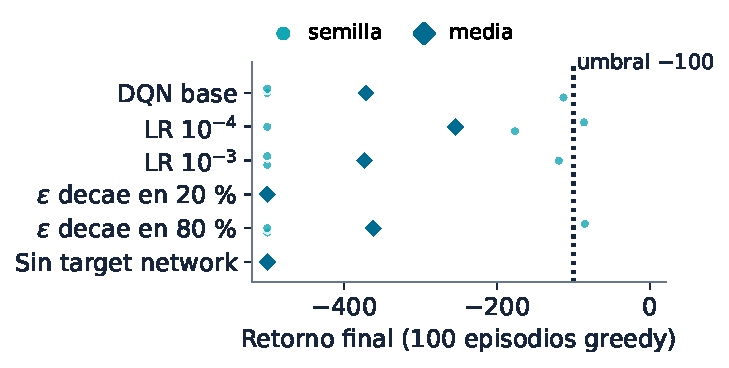
\includegraphics[width=\linewidth,height=.45\textheight,keepaspectratio]{figs/fig_acrobot.pdf}\par\vspace{.05cm}
{\color{Muted}\scriptsize Retorno final por semilla y media de cada variante de DQN.}
\column{.40\textwidth}
\footnotesize\renewcommand{\arraystretch}{1.11}
\begin{tabular}{@{}lrr@{}}\toprule
\textbf{Variante} & \textbf{Media} & \textbf{Éxitos}\\\midrule
DQN base & $-371{,}05$ & 0/3\\
\rowcolor{Sky!45}LR $10^{-4}$ & \textbf{$-254{,}25$} & 1/3\\
LR $10^{-3}$ & $-373{,}04$ & 0/3\\
$\epsilon$ 20\% & $-500{,}00$ & 0/3\\
$\epsilon$ 80\% & $-361{,}72$ & 1/3\\
Sin target & $-500{,}00$ & 0/3\\\bottomrule
\end{tabular}
\vspace{.12cm}
\begin{info}\small Se varía \textbf{un factor a la vez} y se conservan las tres semillas, incluidas las fallidas.\end{info}
\end{columns}
\vspace{.10cm}
\begin{takeaway}\small\textbf{Hallazgo:} LR $10^{-4}$ mejoró la media sin éxito generalizado. El decaimiento rápido de exploración terminó en $-500$ en las tres semillas.\end{takeaway}
\end{frame}

% 7 — 0:55
\begin{frame}{Ablación: ¿qué sucede sin red objetivo?}
\begin{columns}[T,onlytextwidth]
\column{.48\textwidth}
\begin{info}
\textbf{DQN con target network}\par\vspace{.13cm}
{\centering\color{Blue}\fontsize{27}{30}\selectfont\bfseries $-371{,}05$\par}
\vspace{.06cm}
\small Media final entre las 3 semillas; ninguna alcanzó el umbral.
\end{info}
\column{.48\textwidth}
\begin{info}
\textbf{DQN sin target network}\par\vspace{.13cm}
{\centering\color{Warn}\fontsize{27}{30}\selectfont\bfseries $-500{,}00$\par}
\vspace{.06cm}
\small Resultado final idéntico para las tres semillas; 0/3 éxitos.
\end{info}
\end{columns}
\vspace{.15cm}
\begin{takeaway}
\textbf{Interpretación:} mantener una copia más estable de los valores objetivo se asocia con mejor rendimiento en este diseño. El \emph{replay buffer} siguió activo durante la ablación.
\end{takeaway}
\vspace{.09cm}
{\footnotesize\color{Muted} Precaución: no se demuestra superioridad universal ni un mecanismo causal de inestabilidad.}
\end{frame}

% 8 — 1:10
\begin{frame}{Tier 3 · Double DQN: mejora media, no robusta}
\begin{columns}[T,onlytextwidth]
\column{.51\textwidth}
\centering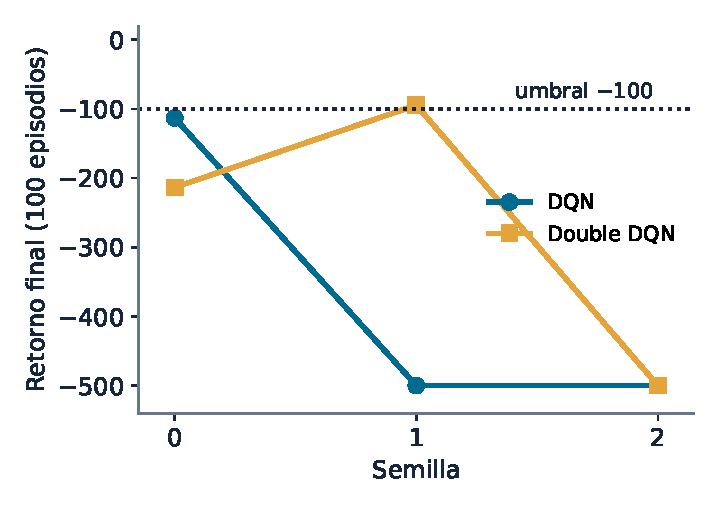
\includegraphics[width=\linewidth,height=.55\textheight,keepaspectratio]{figs/fig_double_dqn.pdf}
\column{.47\textwidth}
\footnotesize\renewcommand{\arraystretch}{1.23}
\begin{tabular}{@{}rrrr@{}}\toprule
\textbf{Seed} & \textbf{DQN} & \textbf{DDQN} & \textbf{$\Delta$}\\\midrule
0 & $-113{,}15$ & $-213{,}49$ & $-100{,}34$\\
1 & $-500{,}00$ & $-94{,}64$ & +405,36\\
2 & $-500{,}00$ & $-500{,}00$ & 0,00\\\midrule
\textbf{Media} & $-371{,}05$ & \textbf{$-269{,}38$} & \textbf{+101,67}\\\bottomrule
\end{tabular}
\vspace{.19cm}
\begin{info}
\small Double DQN usa la red \emph{online} para elegir la acción y la red objetivo para valorar esa acción.
\end{info}
\end{columns}
\vspace{.20cm}
\begin{takeaway}\small\textbf{Resultado:} mejora descriptiva de \textbf{101,67 puntos}, pero empeora en una semilla, mejora en otra y empata en la tercera. Con $n=3$ no se puede demostrar superioridad estadística.\end{takeaway}
\end{frame}

% 9 — 0:55
\begin{frame}{Lectura crítica: éxitos, estabilidad y límites}
\begin{columns}[T,onlytextwidth]
\column{.43\textwidth}
\begin{takeaway}\centering
{\color{Blue}\fontsize{30}{32}\selectfont\bfseries 4 / 33}\par
\small ejecuciones superaron su umbral final\par\vspace{.20cm}
{\color{Warn}\Large\bfseries 0 / 11}\par
\small configuraciones exitosas en las tres semillas
\end{takeaway}
\column{.54\textwidth}
\begin{itemize}\RaggedRight\setlength{\itemsep}{.14cm}
\item \textbf{Rendimiento temprano $\neq$ éxito final:} los checkpoints finales pueden ser peores que los intermedios.
\item \textbf{Alta varianza:} solo tres semillas por condición; las medias no establecen superioridad robusta.
\item \textbf{Instrumentación limitada:} no se guardaron curvas de error TD ni valores Q para diagnosticar causas.
\end{itemize}
\end{columns}
\vspace{.16cm}
\begin{info}\small\textbf{Alcance:} Q-learning tabular escala mal con estados continuos; DQN convencional requiere acciones discretas. En locomoción con torques continuos serían más adecuados enfoques como PPO, SAC o TD3 (análisis teórico, no entrenado).\end{info}
\end{frame}

% 10 — 0:50
\begin{frame}{Conclusiones y evidencias reproducibles}
\begin{columns}[T,onlytextwidth]
\column{.61\textwidth}
\begin{info}
\small\textbf{1 · La representación importa.}\par
Q-learning tabular (10 y 20 bins) superó la media final de DQN en CartPole, sin éxito consistente.\par\vspace{.10cm}
\small\textbf{2 · La estabilidad importa.}\par
La red objetivo y la exploración influyeron en Acrobot; las mejoras tempranas no siempre persistieron.\par\vspace{.10cm}
\small\textbf{3 · Double DQN no garantiza convergencia.}\par
Mejoró la media observada, pero los resultados dependieron de la semilla.
\end{info}
\column{.36\textwidth}
\begin{takeaway}
\centering{\color{Blue}\large\bfseries Código + resultados}\par\vspace{.12cm}
\small Repositorio público con \mbox{\textbf{33 JSON}}, \mbox{\textbf{66 CSV}}, \mbox{\textbf{33 checkpoints}} y figuras originales.\par\vspace{.23cm}
\small\href{https://github.com/Steven735-star/rl-benchmark-lab}{github.com/Steven735-star/}\par\small\href{https://github.com/Steven735-star/rl-benchmark-lab}{rl-benchmark-lab}
\end{takeaway}
\end{columns}
\vspace{.12cm}
\begin{info}\small\textbf{Idea clave:} un buen resultado en una ejecución no implica aprendizaje estable. \textbf{Trabajo futuro:} más semillas, diagnóstico de valores Q y validación independiente de checkpoints.\end{info}
\end{frame}

\end{document}
